\section{Language Definition}
\label{sec:language_def}

\subsection{A Typical Transformation}

Most \emph{DSLTrans} transformations have a common subset of elements. Figure
\ref{fig:example_transformation_structure} shows some of those. Usually there is
one \emph{FilePort} that points to some input model \emph{XMI} file and contains
a \emph{MetaModelIdentifier} that references the metamodel of the input model so
\emph{DSLTrans} can validate the input. Then there are multiple \emph{Layers},
connected using a \emph{PreviousSource} association. Each \emph{Layer} can have
an output model and must have a \emph{MetaModelIdentifier} and various
\emph{Rules}. Every \emph{Rule} has a \emph{MatchModel} and an
\emph{ApplyModel}, each with the match and the apply pattern respectively.

\begin{figure}[h]
\begin{center}
  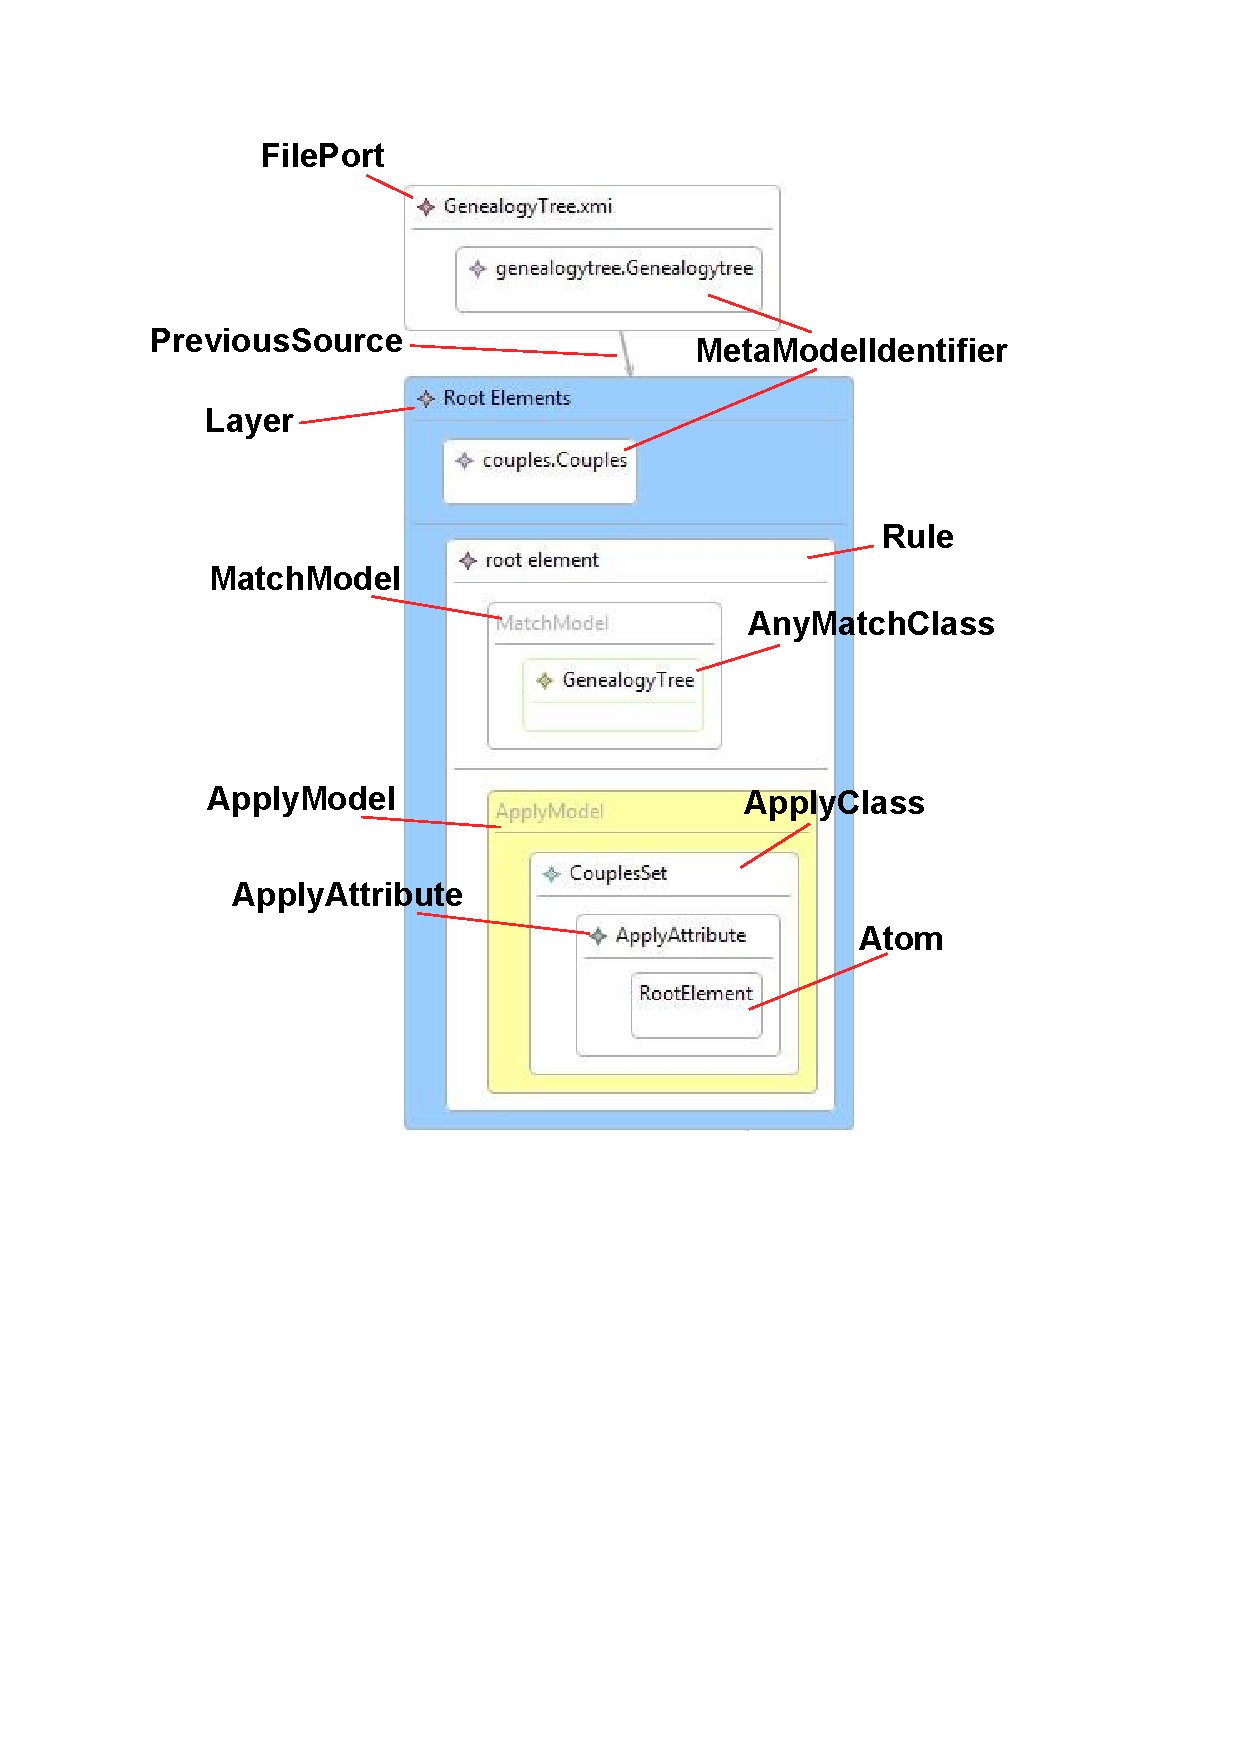
\includegraphics[scale=0.6, trim=2.3cm 10.2cm 3.6cm 2.2cm,
  clip]{imgs/example_transformation_structure.pdf}
  \caption{Example transformation structure.}
  \label{fig:example_transformation_structure}
\end{center}
\end{figure}

% TODO Place here a print of a simple transformation in the textual syntax.

% TODO Criar aqui um flowchart com a semantica do DSLTrans feito por mim. 
% \subsection{\emph{DSLTranslator} Engine}

\clearpage

\subsection{Language Constructs}

Bellow is the description of each \emph{DSLTrans} element along with its
representation in both visual and textual concrete syntaxes.


% Aqui ficam varias subseccoes que abordam cada elemento recorrendo se
% necessario a varios exemplos para mostrar o seu uso.

% Os exemplos podem ser varias consultas possiveis a tirar do modelo
% GenealogyTree

\subsubsection{Objects}

\paragraph{AnyMatchClass}

The \emph{AnyMatchClass} is used in a \emph{MatchModel} to
capture \emph{all} the elements in the input model. When used within a more
complex pattern the set of matched elements can be reduced. Figure
\ref{fig:any_match_class_example} shows an example where all the
\emph{Marriage} elements are being captured and in figure
\ref{fig:any_match_class_example_attr} only those whose attribute \emph{name}
has the value \emph{Thomas-Sarah} are matched.

\begin{center}
  \begin{tabular}{ | c | p{\paragraphsize} | }
    \hline
    \textbf{Property} & \textbf{Description} \\ \hline
    Class Name & Type or Class of the element to be matched.  \\ \hline
    Description & A meaningful description should be used for documentation
  purposes. \\ \hline
    Package Name & This is a very important property that should always be
  correctly set. You can find the
  correct value by looking to the corresponding metamodel's root package as
  shown in figure \ref{fig:ecore_root_package}. \\ \hline
  \end{tabular}
\end{center}

% TODO Here goes a textual syntax print alongside the visual print.
\begin{figure}[h]
\begin{center}
  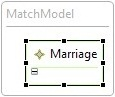
\includegraphics[scale=0.7]{imgs/any_match_class_example.jpg}
  \caption{AnyMatchClass example.}
  \label{fig:any_match_class_example}
\end{center}
\end{figure}


\begin{figure}[h]
\begin{center}
  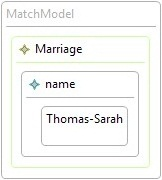
\includegraphics[scale=0.7]{imgs/any_match_class_example_attr.jpg}
  \caption{AnyMatchClass example combined with MatchAttribute and Atom.}
  \label{fig:any_match_class_example_attr}
\end{center}
\end{figure}

\begin{figure}[h]
\begin{center}
  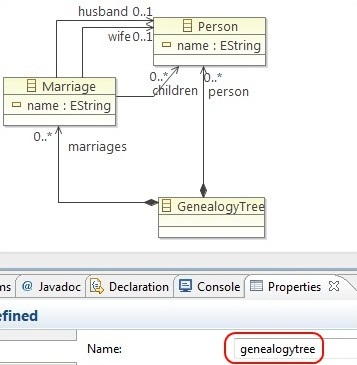
\includegraphics[scale=0.7]{imgs/ecore_root_package.jpg}
  \caption{Root package name property.}
  \label{fig:ecore_root_package}
\end{center}
\end{figure}



\paragraph{ApplyAttribute}

\emph{ApplyAttributes} are inserted inside \emph{ApplyClasses} either to specify
an attribute value or to capture a previously generated element with some attribute
value (if used in an \emph{ApplyClass} connected with a
\emph{PositiveBackwardRestriction}). Figure \ref{fig:import_existing_couples}
shows one \emph{ApplyAttribute} with no name specified. This is usually used to
tell \emph{DSLtranslator} to keep traces in memory so that the generated element
(in this case, a \emph{Couple}) can be later referenced.

\begin{center}
  \begin{tabular}{ | c | p{\paragraphsize} | }
    \hline
    \textbf{Property} & \textbf{Description} \\ \hline
    Attribute Name & Name of the attribute to be applied.  \\ \hline
    Description & A meaningful description should be used for documentation
  purposes. \\ \hline
  \end{tabular}
\end{center}


\paragraph{ApplyClass}

The \emph{ApplyClass} is used to created new elements in the apply patterns or
match previously generated elements (if used with a
\emph{PositiveBackwardRestriction}).

Figure \ref{fig:import_existing_couples} shows an \emph{ApplyClass} named
\emph{Couple}.


\begin{center}
  \begin{tabular}{ | c | p{\paragraphsize} | }
    \hline
    \textbf{Property} & \textbf{Description} \\ \hline
    Class Name & Type or Class of the element to be applied.  \\ \hline
    Description & A meaningful description should be used for documentation
  purposes. \\ \hline
    Group Name & This property helps you to organize your \emph{ApplyClasses}
  by groups if you want.  \\ \hline
    Package Name & This is a very important property that should always be
  correctly set. You can find the
  correct value by looking to the corresponding metamodel's root package as
  shown in figure \ref{fig:ecore_root_package}. \\ \hline
  \end{tabular}
\end{center}

\paragraph{ApplyModel}

An \emph{ApplyModel} is just a container for the pattern to apply in case a
match is found. Figure \ref{fig:rule_example} shows one.



\subsubsection{Atom}

\emph{Atoms} are usually used inside \emph{MatchAttributes} and
\emph{ApplyAttributes}  to express arbitrary values. Figure
\ref{fig:matchattribute_with_atom} shows an \emph{Atom} inside a
\emph{MatchAttribute} and figure \ref{fig:match_attrbute_copy} an \emph{Atom}
combined with an \emph{ApplyAttribute}. 

\begin{center}
  \begin{tabular}{ | c | p{\paragraphsize} | }
    \hline
    \textbf{Property} & \textbf{Description} \\ \hline
    Value & Value that the \emph{Atom} represents. \\ \hline
  \end{tabular}
\end{center}

\paragraph{AttributeRef}

The \emph{AttributeRef} element is used to copy some attribute value from a
matched element to an applied one. Figure \ref{fig:atribute_ref_concat_atoms}
shows an \emph{AttributeRef} inside the second part of a \emph{Concat} together
with the \emph{AttributeRef (Connection)} that points to the attribute being
copied.



\paragraph{Concat}

The \emph{Concat} concatenates \emph{Atoms}, \emph{AttributeRefs} and
\emph{WildCards} inside \emph{ApplyAttributes} allowing for a flexible value
 manipulation. Figure \ref{fig:atribute_ref_concat_atoms} shows a
\emph{Concat} element combined with an \emph{Atom} and an \emph{AttributeRef} to
give the ``Dr.'' title to every \emph{Person}. In figure
\ref{fig:concat_wild_card} shows a complex apply pattern that captures all
\emph{Person} elements that generated new \emph{Person} whose name starts with
``J''. It combines a \emph{Concat} with an \emph{Atom} and a \emph{WildCard}.

\begin{figure}[h]
\begin{center}
  \subfloat[Concat
  with
  AttributeRef
  example.]{\label{fig:atribute_ref_concat_atoms}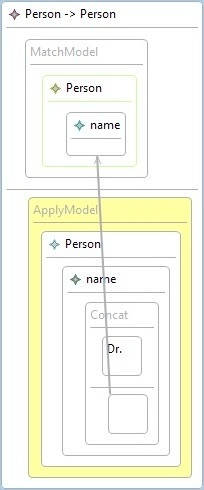
\includegraphics[scale=0.7]{imgs/atribute_ref_concat_atoms.jpg}}
  \subfloat[Concat
  and
  wildcard
  example.]{\label{fig:concat_wild_card}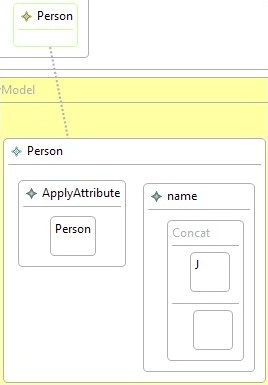
\includegraphics[scale=0.7]{imgs/concat_wild_card.jpg}}
  \caption{}
  \label{fig:concat_examples}
\end{center}
\end{figure}



\paragraph{ExistsMatchClass}

As the \emph{AnyMatchClass} element, the \emph{ExistsMatchClass} is also used to
create match patterns but it only cares about finding one element, not all of
them. It can be combined with \emph{MatchAttributes} to further refine the
element to be matched. Figure \ref{fig:pattern_exists_match_class} shows an
example of a pattern with an \emph{ExistMatchClass}. Beware that when combining
an \emph{ExistMatchClass} and an \emph{AnyMatchClass}, the \emph{AnyMatchClass}
will always prevail over the \emph{ExistMatchClass} no matter what the direction
of the association between them. For instance, in pattern
\ref{fig:pattern_exists_match_class} the intention is to capture 
\emph{every Marriage} with a \emph{wife}, not \emph{only one Person} 
that is a \emph{wife} in every \emph{Marriage}.

\begin{center}
  \begin{tabular}{ | c | p{\paragraphsize} | }
    \hline
    \textbf{Property} & \textbf{Description} \\ \hline
    Class Name & Type or Class of the element to be matched.  \\ \hline
    Description & A meaningful description should be used for documentation
  purposes. \\ \hline
    Package Name & This is a very important property that should always be
  correctly set. You can find the
  correct value by looking to the corresponding metamodel's root package as
  shown in figure \ref{fig:ecore_root_package}. \\ \hline
  \end{tabular}
\end{center}

\begin{figure}[h]
\begin{center}
  \subfloat[Two
  AnyMatchClasses]{\label{fig:pattern_any_match_class}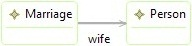
\includegraphics[scale=0.7]{imgs/pattern_any_match_class.jpg}}
  \subfloat[Equivalent pattern
using
an
AnyMatchClass
and
an
ExistMatchClass.]{\label{fig:pattern_exists_match_class}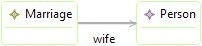
\includegraphics[scale=0.7]{imgs/pattern_exists_match_class.jpg}}
  \caption{}
  \label{fig:match_models_examples_2}
\end{center}
\end{figure}



\paragraph{FilePort}

The \emph{FilePort} element represents an input model. A
transformation can have multiple \emph{FilePorts} if it uses multiple input
models. An input model always has to conform to a metamodel, that is why the
\emph{FilePort} always contains a \emph{MetaModelIdentifier} element to tell
\emph{DSLTranslator} which metamodel the input model conforms to. Figure
\ref{fig:FilePort} shows an example of a \emph{FilePort} and its
\emph{MetaModelIdentifier}. 

\begin{center}
  \begin{tabular}{ | c | p{\paragraphsize} | }
    \hline
    \textbf{Property} & \textbf{Description} \\ \hline
    File Path URI & A meaningful name for the current input.   \\ \hline
  \end{tabular}
\end{center}

% TODO Here goes a textual syntax print alongside the visual print.
\begin{figure}[h]
\begin{center}
  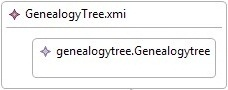
\includegraphics[scale=0.7]{imgs/FilePort.jpg}
  \caption{FilePort example.}
  \label{fig:FilePort}
\end{center}
\end{figure}


\paragraph{Layer}

\emph{Layers} establish an order to the transformation execution. A
transformation can have several sequential \emph{Layers} or even parallel ones if
its purpose is to produce more than one output model. Each \emph{Layer} has a
\emph{PreviousSource} association that connects it to another \emph{Layer} or a
\emph{FilePort}. Figure \ref{fig:layer_mmid_model_apmodel} shows an example of a
\emph{Layer}.

\begin{center}
  \begin{tabular}{ | c | p{\paragraphsize} | }
    \hline
    \textbf{Property} & \textbf{Description} \\ \hline
    Description & Here you write a brief description on what the \emph{Layer}
  is supposed to do.  \\ \hline
    Group Name & This property helps you to organize your \emph{Layers} by
  groups if you want. \\ \hline
    Name & A symbolic name for the \emph{Layer}. \\ \hline
    Output File Path URI & The relative or absolute path for the resulting
  model of the current \emph{Layer}. \\ \hline
    Previous Source & This property is automatically filled if you insert the
  \emph{PreviousSource} connection but if you prefer you can set it manually by
  writing the name of the previous \emph{Layer} or \emph{FilePort} here. \\ \hline
  \end{tabular}
\end{center}

\paragraph{MatchAttribute}

The \emph{MatchAttribute} element is used when it is necessary to capture some
element's attribute value or to match an element with a specific attribute
value. Figure \ref{fig:matchattribute_with_atom} shows the \emph{MatchAttribute}
element being used to say that only the \emph{Person} elements whose name is
John are matched and figure \ref{fig:match_attrbute_copy} illustrates a way to
copy an attribute value between match and apply elements by combining the
\emph{MatchAttribute} with \emph{ApplyAttribute} and \emph{AttributeRef}.


\begin{figure}[h]
\begin{center}
  \subfloat[MatchAttribute with an AttributeRef
  example]{\label{fig:match_attrbute_copy}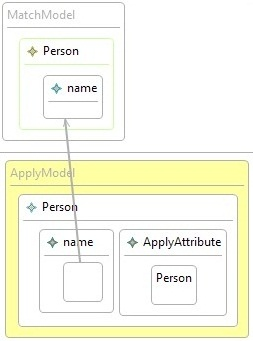
\includegraphics[scale=0.7]{imgs/match_attrbute_copy.jpg}}
  \subfloat[MatchAttribute with an Atom
  example.]{\label{fig:matchattribute_with_atom}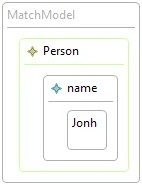
\includegraphics[scale=0.7]{imgs/matchattribute_with_atom.jpg}}
  \caption{}
  \label{fig:match_attribute_examples}
\end{center}
\end{figure}

\begin{center}
  \begin{tabular}{ | c | p{\paragraphsize} | }
    \hline
    \textbf{Property} & \textbf{Description} \\ \hline
    Attribute Name & Name of the attribute to be matched.  \\ \hline
    Description & A meaningful description should be used for documentation
  purposes. \\ \hline
  \end{tabular}
\end{center}

\paragraph{MatchModel}

The \emph{MatchModel} contains a \emph{Rule's} match pattern (see figure
\ref{fig:rule_example}). There can be multiple \emph{MatchModels} in the same
\emph{Rule} although it is rare: one can actually override the
\emph{PreviousSource} connection of a \emph{MatchModel} by setting it's
\emph{ExplicitSource} property or by creating an \emph{ExplicitSource}
connection to some \emph{FilePort}. Figures \ref{fig:match_models_sperated} and
\ref{fig:match_model_equivalent} illustrate two equal patterns but the left one
is split across two \emph{MatchModels}. This does not seem very useful and
it isn't but when combined with the \emph{ExplicitSource} property lets you
parametrize transformations (see section \ref{subsec:fda_execution}).

\begin{figure}[h]
\begin{center}
  \subfloat[Two
  separated
  MatchModels]{\label{fig:match_models_sperated}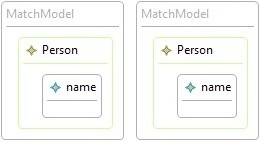
\includegraphics[scale=1]{imgs/match_models_sperated.jpg}}
\subfloat[Equivalent
pattern
in
a
single
MatchModel.]{\label{fig:match_model_equivalent}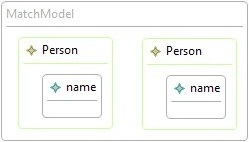
\includegraphics[scale=1]{imgs/match_model_equivalent.jpg}}
  \caption{MatchModel examples.}
  \label{fig:match_models_examples}
\end{center}
\end{figure}

\begin{center}
  \begin{tabular}{ | c | p{\paragraphsize} | }
    \hline
    \textbf{Property} & \textbf{Description} \\ \hline
    Explicit Source & Name of a \emph{FilePort} to get an input model from.  \\ \hline
  \end{tabular}
\end{center}

\paragraph{MetaModelIdentifier}

The \emph{MetaModelIdentifier} element is used inside \emph{FilePorts} and
\emph{Layers} to refer to the relevant metamodels. Wherever there is an input or
output model, the \emph{MetaModelIdentifier} has to be there. Figure
\ref{fig:FilePort} shows a \emph{MetaModelIdentifier} inside a \emph{FilePort}
and figure \ref{fig:layer_mmid_model_apmodel} illustrates it in a \emph{Layer}
because a \emph{Layer} can generate an output model.

\begin{center}
  \begin{tabular}{ | c | p{\paragraphsize} | }
    \hline
    \textbf{Property} & \textbf{Description} \\ \hline
    Meta Model Name & Specifies the name of the metamodel. This name usually
  takes the form of the \verb=root_package_name.Root_package_name= as you have
  seen in section \ref{sec:quick_start}.  \\ \hline
    Meta Model URI & The relative or absolute path to the metamodel. \\ \hline
  \end{tabular}
\end{center}

\begin{figure}[h]
\begin{center}
  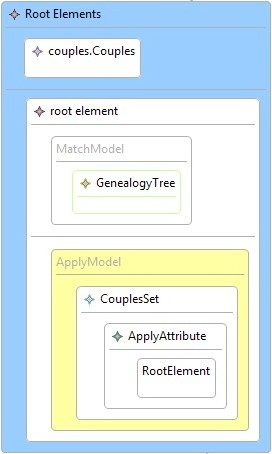
\includegraphics[scale=0.7]{imgs/layer_mmid_model_apmodel.jpg}
  \caption{Layer with MetaModelIdentifier example.}
  \label{fig:layer_mmid_model_apmodel}
\end{center}
\end{figure}




\paragraph{NegativeMatchClass}

The \emph{NegativeMatchClass} is mostly used in combination with a
\emph{NegativeMatchAssotiation} to express that you don't want an element to
exist in some pattern. In figure \ref{fig:negative_marriage_example} the pattern
captures all \emph{Person} objects that are not children, i. e., it will match
all root elements.


\begin{center}
  \begin{tabular}{ | c | p{\paragraphsize} | }
    \hline
    \textbf{Property} & \textbf{Description} \\ \hline
    Class Name & Type or Class of the element to be matched.  \\ \hline
    Description & A meaningful description should be used for documentation
  purposes. \\ \hline
    Package Name & This is a very important property that should always be
  correctly set. You can find the
  correct value by looking to the corresponding metamodel's root package as
  shown in figure \ref{fig:ecore_root_package}. \\ \hline
  \end{tabular}
\end{center}


\begin{figure}[h]
\begin{center}
  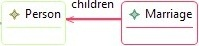
\includegraphics[scale=0.7]{imgs/negative_marriage_example.jpg}
  \caption{NegativeMatchClass example.}
  \label{fig:negative_marriage_example}
\end{center}
\end{figure}



\paragraph{Rule}

\emph{Rules} are inserted inside each \emph{Layer} and they contain a match side
and an apply side. Figure \ref{fig:rule_example} shows an example rule already
filled with some elements. A \emph{Rule} always needs to contain at least a
\emph{Match} and an \emph{Apply} models.

\begin{figure}[h]
\begin{center}
  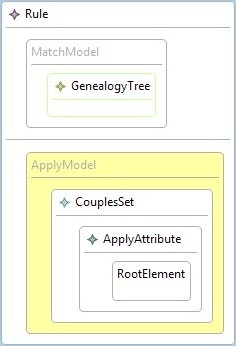
\includegraphics[scale=0.7]{imgs/rule_example.jpg}
  \caption{Example rule containing a MatchModel, ApplyModel, AnyMatchClass and
  ApplyClass along with attributes.}
  \label{fig:rule_example}
\end{center}
\end{figure}


\begin{center}
  \begin{tabular}{ | c | p{\paragraphsize} | }
    \hline
    \textbf{Property} & \textbf{Description} \\ \hline
    Description & Use this property to describe the purpose of the
  rule if you want.  \\
    \hline
  \end{tabular}
\end{center}


\paragraph{Wildcard}

\emph{Wildcards} are used most frequently inside \emph{ApplyAttributes},
combined with \emph{Atoms} and \emph{Concats} to restrict the number of matched
elements that where previously generated\footnote{This means the
\emph{ApplyClass} has to be connected to some match class with a
\emph{PositiveBackwardRestriction.}}. Figure \ref{fig:concat_wild_card} shows an
example of a pattern that will only be applied to \emph{Person} elements that
where previously generated and whose name starts with a ``J''. A \emph{Wildcard}
represents any value.

% TODO isNull is crazy :o
%\subsubsection{isNull}


%%% END OF OBJECTS

\subsubsection{Connections}

\paragraph{ApplyAssociation}

\emph{ApplyAssociations} always generate relations between \emph{ApplyClasses}
in the output model. Notice that they cannot be used to capture previously
generated elements as \emph{ApplyAttributes} can do. Figure
\ref{fig:connect_imported_couples} shows an \emph{ApplyAssociation} between a
\emph{CouplesSet} and a \emph{Couple}.


\begin{center}
  \begin{tabular}{ | c | p{\paragraphsize} | }
    \hline
    \textbf{Property} & \textbf{Description} \\ \hline
    Association Name & The name of the association. This depends on the input
  metamodel.  \\
    \hline
  \end{tabular}
\end{center}


\paragraph{AttributeRef}

The \emph{AttributeRef} connection points to a \emph{MathAttribute} to copy its
value (see figure \ref{fig:atribute_ref_concat_atoms}).



\paragraph{ExplicitSource}

The \emph{ExplicitSource} allows the user to connect a \emph{MatchModel}
directly to a \emph{FilePort} and match a pattern against an input model.
Figure \ref{fig:explicit_source_example} shows an example of an
\emph{ExplicitSource} connection (it's the thin line between the
\emph{MatchModel} and the \emph{FilePort}).

\begin{figure}[h]
\begin{center}
  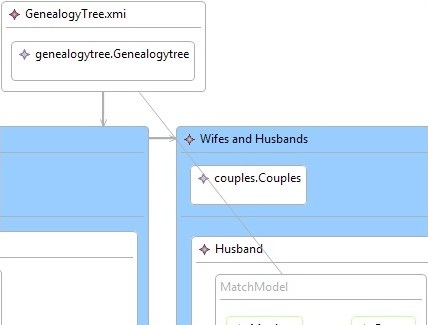
\includegraphics[scale=0.7]{imgs/explicit_source_example.jpg}
  \caption{ExplicitSource example.}
  \label{fig:explicit_source_example}
\end{center}
\end{figure}






\paragraph{Import}

Using the \emph{Import} element, the user is capable of copying an entire tree
of elements from an input model to an output model by matching the tree's root
element. \emph{DSLTranslator} will copy the element along with its attributes
and descendants, keeping all the relations that belong to the tree. Beware that
if any of the imported elements has an association referring other element that
does not belong to the tree (i. e., is not a descendant of the root
matched element), that connection will cease to exist.
Naturally, all imported elements must conform to the same metamodel as the
output model. For instance, if you already had a \emph{CouplesHierarchy} model
(like the one shown in figure \ref{fig:existing_couples_hierarchy}) and you
wanted to create a new model (as the one in figure
\ref{fig:couples_hierarchy_extended}) that extends it with information from a
\emph{GenealogyTree} model , you could use an \emph{Import} to copy the
\emph{Frank-Basie} couple along with its child couples and then attach the
imported tree to the output model like figures \ref{fig:import_existing_couples}
and \ref{fig:connect_imported_couples} illustrate. The \emph{MatchModels} that
capture the imported elements are directly connected to \emph{FilePort} that
points to the existing \emph{Couples} model shown in figure
\ref{fig:existing_couples_hierarchy}.

\begin{figure}[h]
\begin{center}
  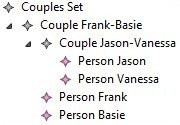
\includegraphics[scale=0.7]{imgs/existing_couples_hierarchy.jpg}
  \caption{Couples Hierarchy model.}
  \label{fig:existing_couples_hierarchy}
\end{center}
\end{figure}

\begin{figure}[h]
\begin{center}
  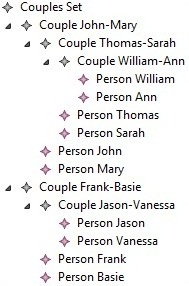
\includegraphics[scale=0.7]{imgs/couples_hierarchy_extended.jpg}
  \caption{Couples Hierarchy extended model.}
  \label{fig:couples_hierarchy_extended}
\end{center}
\end{figure}


\begin{figure}[h]
\begin{center}
  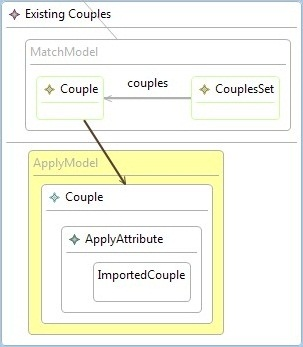
\includegraphics[scale=0.7]{imgs/import_existing_couples.jpg}
  \caption{Import existing couples tree rule.}
  \label{fig:import_existing_couples}
\end{center}
\end{figure}

\begin{figure}[h]
\begin{center}
  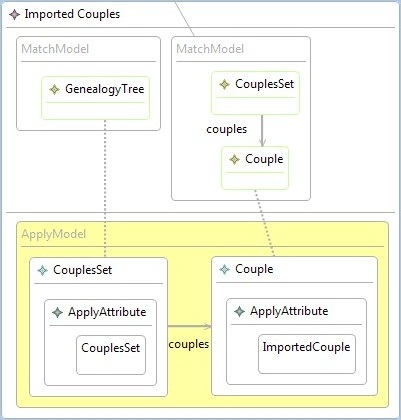
\includegraphics[scale=0.7]{imgs/connect_imported_couples.jpg}
  \caption{Connect imported couples tree rule.}
  \label{fig:connect_imported_couples}
\end{center}
\end{figure}



% TODO Bruno vai esclarecer no email.
% \paragraph{NegativeBackwardRestriction}




\paragraph{NegativeIndirectAssociation}

The \emph{NegativeIndirectAssociation} is used to create patterns where a
containment association of any depth between two connected elements cannot
exist. It usually is combined with a \emph{NegativeMatchClass} to capture
elements that are not contained in other elements by any depth. Figure
\ref{fig:neg_indir_assoc_example} shows a pattern with the same meaning of the
one shown in figure \ref{fig:negative_match_class_and_assoc} but disregarding
the containment association's name.

\begin{figure}[h]
\begin{center}
  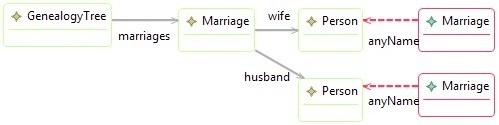
\includegraphics[scale=0.7]{imgs/neg_indir_assoc_example.jpg}
  \caption{Negative Indirect Associations together with Negative Match Classes.}
  \label{fig:neg_indir_assoc_example}
\end{center}
\end{figure}

\begin{center}
  \begin{tabular}{ | c | p{\paragraphsize} | }
    \hline
    \textbf{Property} & \textbf{Description} \\ \hline
    Association Name & This can be any name you want.  \\
    \hline
  \end{tabular}
\end{center}


\paragraph{NegativeMatchAssociation}

As the \emph{PositiveMatchAssociation}, the \emph{NegativeMatchAssociation} is
used to connect match classes allowing for more complex match patterns. Unlike
the \emph{PositiveMatchAssociation}, it expresses that an association must not
exist between two elements and it is often combined with a
\emph{NegativeMatchClass} to say that an element cannot exist in some pattern.
Figure \ref{fig:negative_match_class_and_assoc} shows an example where
\emph{Persons} (and respective \emph{Marriages}) that have no parents are being
matched.

\begin{center}
  \begin{tabular}{ | c | p{\paragraphsize} | }
    \hline
    \textbf{Property} & \textbf{Description} \\ \hline
    Association Name & The name of the association. This depends on the input
  metamodel.  \\
    \hline
  \end{tabular}
\end{center}

\begin{figure}[h]
\begin{center}
  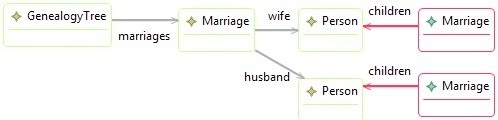
\includegraphics[scale=0.7]{imgs/negative_match_class_and_assoc.jpg}
  \caption{Negative Match Associations together with Negative Match Classes.}
  \label{fig:negative_match_class_and_assoc}
\end{center}
\end{figure}



\paragraph{PositiveBackwardRestriction}

The \emph{PositiveBackwardRestriction} association is used to generate
associations between output model elements generated in previous layers. It
connects match elements to apply elements in order to match the generated and
generator elements. For instance, in figure
\ref{fig:positive_backward_restriction_example} a new relation named
\emph{husband} is being created between any \emph{Couple} and \emph{Person} that
were previously created and whose creators (\emph{Marriage} and \emph{Person})
are related by the \emph{husband} association.


\begin{figure}[h]
\begin{center}
  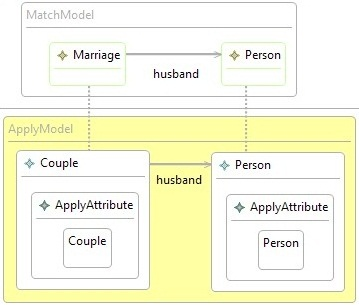
\includegraphics[scale=0.7]{imgs/positive_backward_restriction_example.jpg}
  \caption{Positive Backward Restriction example.}
  \label{fig:positive_backward_restriction_example}
\end{center}
\end{figure}



\paragraph{PositiveIndirectAssociation}

The \emph{PositiveIndirectAssociation} is used to abstract long containment
relationships\footnote{Long containment relationships mean that there can be
several elements in between.} between two elements. For instance, in the
\emph{GenealogyTree} metamodel, the association \emph{marriages} between a
\emph{GenealogyTree} and a \emph{Marriage} is a 1-level containment and the
pattern shown in figure \ref{fig:positive_indirect_assoc} matches the two
elements. But what if the metamodel allowed \emph{Marriages} inside
\emph{Marriages} by adding an containment association between \emph{Marriage}
elements? The resulting models could have long lists of \emph{Marriages} inside
\emph{Marriages}, all connected with containment relationships. In that
scenario, the pattern shown in figure \ref{fig:indirect_assoc_marriages} would
match all \emph{Marriages} inside the \emph{John-Mary} \emph{Marriage}. Notice
that all containment relations (of any depth) will be matched, even if they
haven't got the same name.

\begin{figure}[h]
\begin{center}
  \subfloat[Positive Indirect Association
  between
  GenealogyTree
  and
  Marriage.]{\label{fig:positive_indirect_assoc}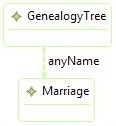
\includegraphics[scale=0.7]{imgs/positive_indirect_assoc.jpg}}
  \subfloat[Positive Indirect Association
  between
  Marriages.]{\label{fig:indirect_assoc_marriages}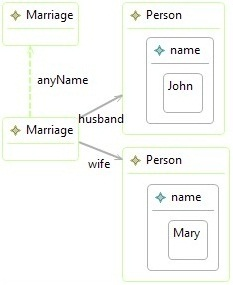
\includegraphics[scale=0.7]{imgs/indirect_assoc_marriages.jpg}}
  \caption{}
  \label{fig:positive_indirect_assoc_examples}
\end{center}
\end{figure}


\begin{center}
  \begin{tabular}{ | c | p{\paragraphsize} | }
    \hline
    \textbf{Property} & \textbf{Description} \\ \hline
    Association Name & This can be any name you want. \\
    \hline
  \end{tabular}
\end{center}


\paragraph{PositiveMatchAssociation}

It is often necessary to create match patterns with more than one element. The
\emph{PositiveMatchAssociation} is a possible connection between two match
classes that expresses that a relation has to exist between those elements in
the input model. In figure \ref{fig:positive_match_example} a \emph{Person} that
is a wife and a child simultaneously is being matched; on the other hand, the
rule will not be applied to a \emph{Person} that is not a child.

\begin{figure}[h]
\begin{center}
  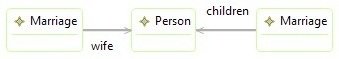
\includegraphics[scale=0.7]{imgs/positive_match_example.jpg}
  \caption{PositiveMatchAssociation examples.}
  \label{fig:positive_match_example}
\end{center}
\end{figure}


\begin{center}
  \begin{tabular}{ | c | p{\paragraphsize} | }
    \hline
    \textbf{Property} & \textbf{Description} \\ \hline
    Association Name & The name of the association. This depends on the input
  metamodel.  \\
    \hline
  \end{tabular}
\end{center}


\paragraph{PreviousSource}

\emph{PreviousSource} is an association that connects a \emph{Layer} to another
\emph{Layer} or \emph{FilePort}. It controls the flow of the transformation.
Figure \ref{fig:two_previous_sources} shows two \emph{PreviousSource}
connections.

\begin{figure}[h]
\begin{center}
  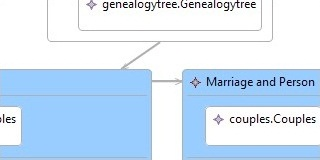
\includegraphics[scale=0.7]{imgs/two_previous_sources.jpg}
  \caption{PreviousSource connections between Layers and FilePort.}
  \label{fig:two_previous_sources}
\end{center}
\end{figure}
